% !TEX root =  ../main.tex 

\section{Personalized schedules for patients in PRIAS}
\label{sec : pers_schedule_PRIAS}
To demonstrate how the personalized scheduling algorithm described in Section \ref{subsubsec : pers_sched_algorithm} works, we apply it to the patients in the PRIAS dataset. To this end, we divide the PRIAS data set into training(5264 patients) and demonstration data sets (3 patients). We fit a joint model to the training data set and then use it to create a personalized schedule for patients in demonstration data set. We fit the joint model using the R package JMbayes \citep{rizopoulosJMbayes}, which uses the Bayesian methodology to estimate the model parameters.

\subsection{Fitting the joint model to PRIAS dataset}
\label{subsec : jm_fit_prias}
The training data set contains information about 5938 prostate cancer patients who satisfied the conditions for enrollment in AS. For every patient the age at the time of induction in AS was recorded. PSA was measured every 3 months for first 2 years and every 6 months thereafter. To detect GR, biopsies were conducted at different time points on the basis of a predetermined schedule as well as PSA-DT as described in Section \ref{sec : introduction}. For the longitudinal analysis of PSA measurements we used $\log_2 PSA$ measurements instead of the raw data. The log transformation was done because the PSA scores took very large values around the time of disease progression. This indicated that the underlying distribution for PSA scores was right skewed. The longitudinal sub-model of the joint model we fit is given by:

\begin{equation*}
\begin{aligned}
\log_2 PSA(t) &= m_i(t) + \varepsilon_i(t), \\
m_i(t) &= (\beta_0 + b_{i0}) + \beta_1 (Age-70) + \beta_2 (Age-70)^2\\ 
&+ \sum_{k=1}^4 \beta_{k+2} B_k(t,\mathcal{K}) + b_{i1} B_7(t, 0.5) + b_{i2} B_8(t, 0.5) \\
\varepsilon_i(t) & \sim N(0, \sigma^2),\\
\boldsymbol{b}_i & \sim N(0, \boldsymbol{D})
\end{aligned}
\end{equation*}

The evolution of PSA levels over time is modeled flexibly using B-splines. For the fixed effects part the spline consists of 3 internal knots. The internal knots are at $\mathcal{K} =\{0.5, 1.2, 2.5\}$ years, and boundary knots are at 0 and 7 years. For the random effects part there is only 1 internal knot at 0.5 years and the boundary knots are at 0 and 7 years. The choice of knots was based on exploratory analysis as well as on the basis of model selection criteria AIC and BIC. The variable Age was median centered to avoid numerical instabilities while estimating the parameters in the model. For the survival sub-model the hazard function we fitted is given by:

\begin{equation}
\label{eq : hazard_prias}
h_i(t) = h_0(t) e^{\gamma_1 (Age-70)  + \gamma_2 (Age-70)^2  \alpha_1 m_i(t) + \alpha_2 m'_i(t)}
\end{equation}
where, $\alpha_1$ and $\alpha_2$ are measures of strength of association between hazard of GR and PSA value $m_i(t)$ and PSA velocity $m'_i(t)$, respectively. $h_0(t)$ is the baseline hazard at time t, and is modeled flexibly using P-splines\citep{eilers1996flexible}. Lastly, to fit the joint model we use the R package JMbayes \cite{rizopoulosJMbayes}, which uses a Bayesian approach for parameter estimation.

\subsubsection{Parameter Estimates}
\label{subsec : param_estimates_jm_fit_prias}
The posterior parameter estimates $p(\boldsymbol{\theta} \mid \mathcal{D}^{PRIAS})$ for the joint model we fitted to the PRIAS data set are shown in Table \ref{tab : PSA_long} and Table \ref{tab : PSA_survival}. Since the longitudinal evolution of $\log_2 PSA$ is modeled with non-linear terms, the interpretation of the coefficients corresponding to time is not straightforward. In lieu of the interpretation we present the fitted evolution of PSA over a period of 10 years for a patient who is 70 years old in Figure \ref{fig : fitted_trend_psa}. It can be seen that the after the first 6 months the PSA levels steadily increase over the follow up period. Since the model for PSA has only additive terms, this evolution remains same for all patients. The effect of Age only affects the baseline PSA score. However it is so small that it can be ignored for all practical purposes.\\

\begin{figure}[!htb]
	\centering
    \captionsetup{justification=centering}
	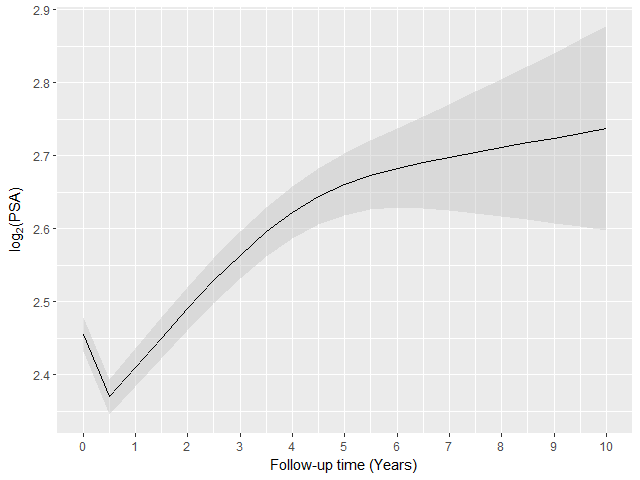
\includegraphics[width=0.8\textwidth]{images/fitted_trend_psa.png}
	\caption{Fitted evolution of $\log_2 PSA$ over a period of 10 years, for a patient who was inducted in AS at the Age of 70 years.}
	\label{fig : fitted_trend_psa}
\end{figure}

\begin{table}[!htb]
\centering
\caption{Longitudinal sub-model estimates for joint model.}
\label{tab : PSA_long}
\captionsetup{justification=centering}
\begin{tabular}{@{}lrrrrr@{}}
\toprule
                                     & Mean   & Std. Dev           & 2.5\%               & 97.5\%              & P              \\ \midrule
Intercept                            &  2.455 & 0.012 & 2.433 & 2.480               & \textless0.000 \\
(Age - 70)                           & 0.003 & 0.001 & 4.9 $\times 10^{-4}$ & 0.006 & 0.032          \\
(Age - 70) $\times$ (Age - 70)       & -0.001 & 1.4 $\times 10^{-4}$ & -0.001 & -3.5 $\times 10^{-4}$ & \textless0.000 \\
Spline: visitTimeYears{[}0, 0.5{]}   & -0.006 & 0.012 & -0.031 & 0.017 & 0.674 \\
Spline: visitTimeYears{[}0.5, 1.2{]} & 0.228 & 0.019 & 0.192 & 0.265               & \textless0.000 \\
Spline: visitTimeYears{[}1.2, 2.5{]} & 0.140 & 0.029 & 0.088 & 0.197               & \textless0.000 \\
Spline: visitTimeYears{[}2.5, 7{]}   & 0.303 & 0.039 & 0.227 & 0.379               & \textless0.000 \\
$\sigma$                               & 0.324 & 0.001 & 0.321 & 0.326              &  \\ \bottomrule
\end{tabular}
\end{table}

For the survival sub-model, the parameter estimates in Table \ref{tab : PSA_survival} show that only $\log_2 PSA$ velocity is strongly associated with hazard of GR. For any patient, a unit increase in $\log_2 PSA$ velocity corresponds to a 11 time increase in hazard of GR. The effect of $\log_2 PSA$ value and effect of Age on hazard of GR are so small that they can be safely ignored for all practical purposes.

\begin{table}[!htb]
\centering
\caption{Survival sub-model estimates for joint model.}
\captionsetup{justification=centering}
\label{tab : PSA_survival}
\begin{tabular}{@{}lrrrrr@{}}
\toprule
Variable                      & Mean   & Std. Dev & 2.5\%  & 97.5\%                 & P              \\ \midrule
Age - 70                      & 0.037 & 0.006 & 0.025 & 0.0490                  & \textless0.000 \\
(Age - 70) $\times$ (Age - 70) & -0.001 & 0.001 & -0.003 & 1.8 $\times 10^{-4}$ & 0.104          \\
$\log_2 PSA$                  & -0.049 & 0.064 & -0.172 & 0.078 & 0.414         \\
Slope: $\log_2 PSA$           & 2.407 & 0.319 & 1.791 & 3.069 & \textless0.000 \\ \bottomrule
\end{tabular}
\end{table}

\subsection{Demonstration of personalized schedules}
In this section, we demonstrate how the personalized scheduling algorithm adapts the time of performing a biopsy according to the PSA history and results from repeat biopsies. The 3 patients we have chosen for the demonstration data set are part of PRIAS program and they have had their repeat biopsies already. Hence a full scale comparison between PRIAS biopsy schedule and personalized scheduling algorithm's biopsy schedule is not possible.\\

The first patient of interest is patient nr. 3174 who was inducted in the PRIAS program at the age of 74 years. Between the last follow up and time of induction there was no repeat biopsy performed for this patient. Hence the predictive distribution $g(T^*_j)$  for this patient depends only on the PSA measurements. For this patient, the evolution of PSA, time of last biopsy and proposed times of biopsies are shown in Figure \ref{fig : prias_demo_pid_3174}. It can be seen that the PSA remains stable for the first 2 years of follow ups, but increases rapidly after that for the next 2 years of follow up. Since the hazard of GR depends on PSA velocity (Table\ref{tab : PSA_survival}), the schedule of biopsy based on personalized scheduling algorithm (Section \ref{fig : sched_algorithm}), adjust the times of biopsy according to the steep rise in PSA profile. At 2 years the expected and median time of GR are 12.5 years and 15.2 years respectively, whereas at 4 years, they are 5.3 and 4 years respectively. It is important to note that the estimates are year 2 are not as useful as the estimates at year 4, because the $Var_g[T^*_j]$ is considerably lower at year 4, as shown in Figure \ref{fig : variance_pred_dist_3174}.\\

\begin{figure}[!htb]
\centering
\captionsetup{justification=centering}
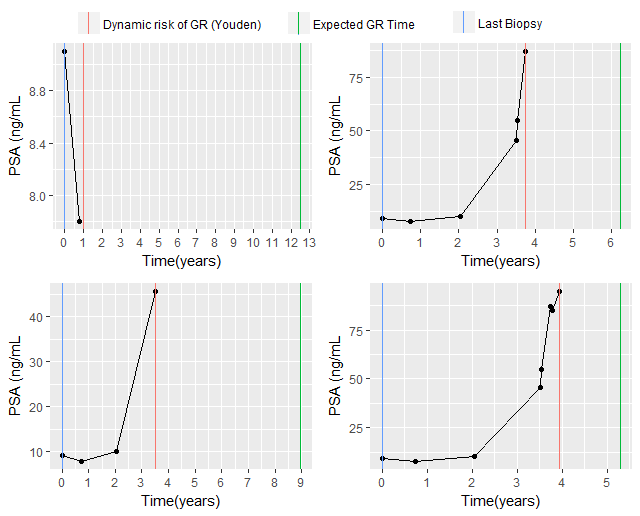
\includegraphics[width=\textwidth]{images/prias_demo/case_3174.png}
\caption{\label{fig : prias_demo_pid_3174} Proposed biopsy times for patient 3174 from PRIAS.}
\end{figure}

The second patient of interest is patient nr. 911. Figure \ref{fig : prias_demo_pid_911} shows the evolution of PSA, time of last biopsy and proposed biopsy times for this patient. Firstly, it can be seen that at between year 1.5 and year 2, the PSA rises sharply, and accordingly the personalized schedules based on expected time of GR preponed the proposed biopsy time from 14.2 years to 13.8 years. The change in median time of GR is trivial. The second observation is that between year 2 and year 3 the PSA decreases sharply and accordingly, the proposed biopsy times are postponed. More specifically the median time of GR increased from 15.2 years at year 2 to 17 years at year 3. Whereas the expected time of GR increased from 13.8 years to 16.6 years. It can also be seen that PSA remains stable up to to year 4. Lastly, because no GR is found at the repeat biopsy performed at 4.1 years, this further leads to postponing of the biopsy times, which become 18.7 and 19.9 for expected time of GR and median time of GR respectively.\\

\begin{figure}[!htb]
\centering
\captionsetup{justification=centering}
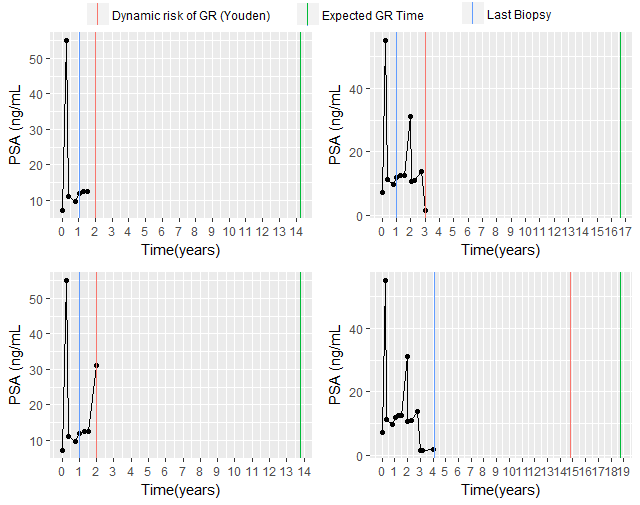
\includegraphics[width=\textwidth]{images/prias_demo/case_911.png}
\caption{\label{fig : prias_demo_pid_911} Proposed biopsy times for patient 911 from PRIAS.}
\end{figure}

The fact that PSA velocity affects the biopsy times is also evident in the case of patient 2340, whose PSA evolution is shown in Figure \ref{fig : prias_demo_pid_2340}. We have purposefully ignored all the biopsies conducted for this patient in PRIAS, to isolate the effect of PSA history. It can be seen that PSA slowly rises to a value of 14 ng/mL over a period of 2.5 years. Correspondingly, there is little change in proposed biopsy times. On the other hand between 2.3 years and 3.3 years the PSA rises very sharply and correspondingly the expected time of GR decreases by an year from 12.5 years to 11.5 years in that period. The median time of GR remains the same though.

\begin{figure}[!htb]
\centering
\captionsetup{justification=centering}
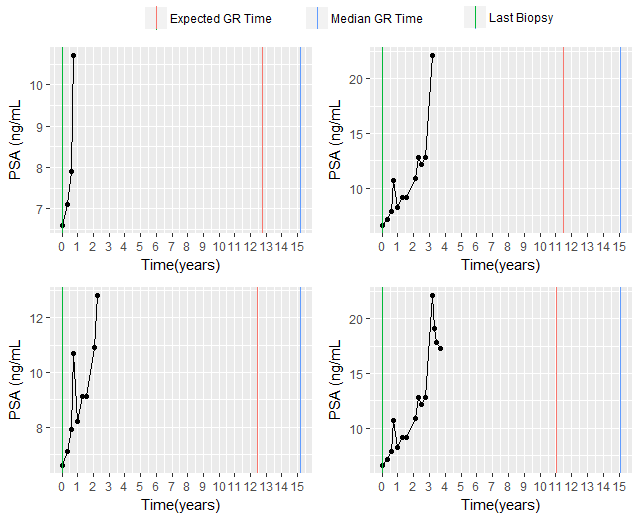
\includegraphics[width=\textwidth]{images/prias_demo/case_2340.png}
\caption{\label{fig : prias_demo_pid_2340} Proposed biopsy times for patient 2340 from PRIAS.}
\end{figure}